\section{What is aging?}

\subsection{Definition and Hallmarks}

\begin{frame}[c]{Aging}
    \large
    
    \begin{block}{Definition}
        Ageing is characterized by a progressive decline in organismal fitness
        occurs with increasing age, ultimately ending in death.
    \end{block}
    \pause
    But how can we measure it?
\end{frame}


\begin{frame}[c]{Hallmarks of Aging}
    According to \cite{lopez2013hallmarks}:
    \begin{itemize}[<+(1)->]
        \item Genomic instability
        \item Telomere attrition
        \item Epigenetic alterations
        \item Loss of proteostasis
        \item Deregulated nutrient-sensing
        \item Mitochondrial dysfunction
        \item Cellular senescence
        \item Stem cell exhaustion
        \item Altered intercellular communication
    \end{itemize}
    \pause
    Hallmarks are mostly just side-effects we can measure!
\end{frame}


\subsection{Common Root Cause Existence}


\begin{frame}[c]{Diabetes: Life Expectancy}
    \large
    Life Expectancy is at least 10 years lower with Diabetes Type 1 \cite{livingstone2015estimated} and about 5 lower less with Type 2.
\end{frame}

\begin{frame}[c]{Cancer: Life Expectancy}
    \large
    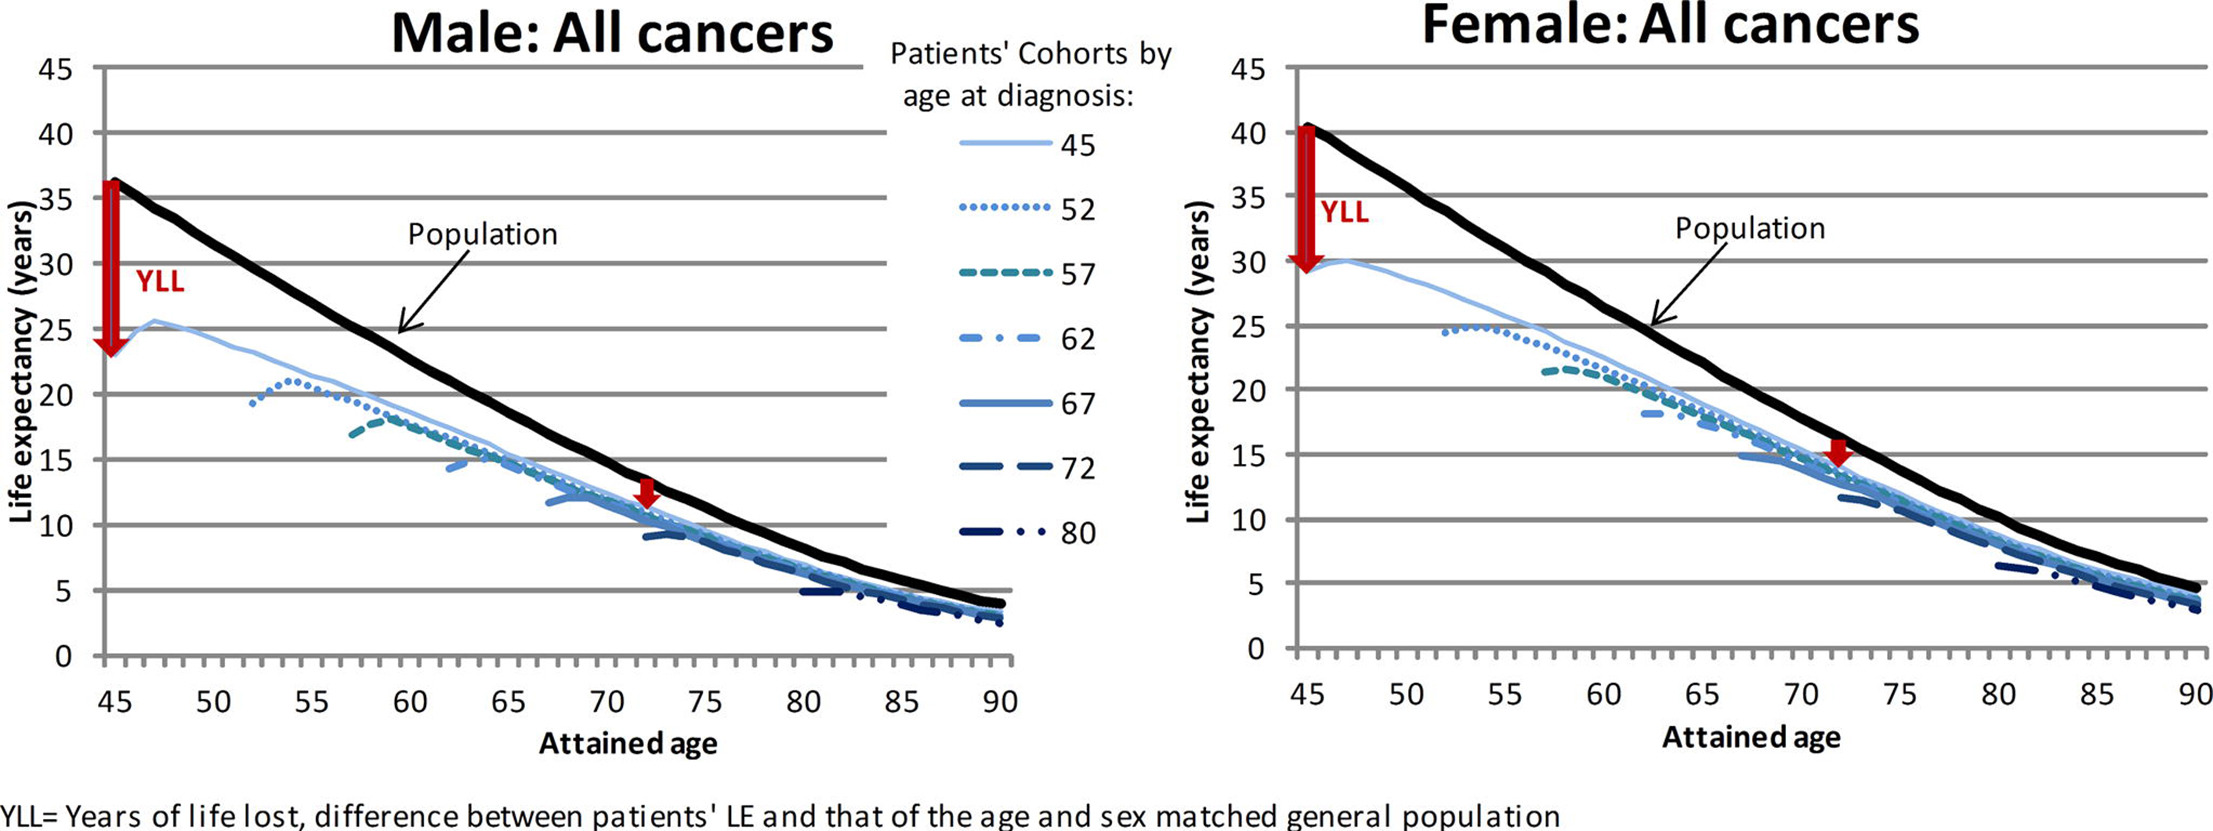
\includegraphics[width=\textwidth]{all_cancers_LE} \\
    \cite{botta2019changes}
\end{frame}


\begin{frame}[c]{Existence proof of common pathways}
    \large
    someone who has one severe illness early is likely to have others \\
\end{frame}


\begin{frame}[c]{Similarity of diseases of aging}
    % \begin{block}{}
    % At the cellular level, a lot of diseases of aging “look similar”, and involve similar pieces. There’s a decrease in cell count, increase in damaged proteins/DNA/fats, and inflammation. We see roughly this pattern in Alzheimers, atherosclerosis, muscle loss, and many others. \cite{CorePath13:online}
    % \end{block}

    \large

    \cite{CorePath13:online}
    At the cellular level:
    \begin{itemize}[<+(1)->]
        \item decrease in cell count
        \item increase in damaged proteins/DNA/fats
        \item inflammation
    \end{itemize}
    \pause

    Roughly this pattern for:
    \begin{itemize}[<+(1)->]
        \item alzheimers
        \item atherosclerosis
        \item muscle loss
        \item many others
    \end{itemize}

\end{frame}



\subsection{Assumed Root Causes}


\begin{frame}[c]{Mitochondrial dysfunction}
    \large
    Turns out, mitochondrial dysfunction accounts for telomere-dependent senescence \cite{passos2007mitochondrial}.
\end{frame}


\begin{frame}[c]
    \large
    Assumed root causes: free radicals and transposon damage \\
    Maybe not in too much detail? Could fill 30min itself \cite{CorePath13:online} \\

    p21 and reactive oxygen feedback for senescence \cite{passos2010feedback}
\end{frame}

